% Created 2021-11-07 So 16:33
% Intended LaTeX compiler: pdflatex
\documentclass[11pt]{article}
\usepackage[utf8]{inputenc}
\usepackage[T1]{fontenc}
\usepackage{graphicx}
\usepackage{longtable}
\usepackage{wrapfig}
\usepackage{rotating}
\usepackage[normalem]{ulem}
\usepackage{amsmath}
\usepackage{amssymb}
\usepackage{capt-of}
\usepackage{hyperref}
\usepackage{lmodern} % Ensures we have the right font
\usepackage[margin=1in]{geometry}
\usepackage{fontspec}
\setmainfont{Arial}
\usepackage[utf8]{inputenc}
\usepackage{graphicx}
\usepackage{amsmath, amsthm, amssymb}
\usepackage[table, xcdraw]{xcolor}
\author{Niklas, Immanuel, Magnus, Fabian}
\date{2021-11-07}
\title{Rassenlehre}
\hypersetup{
 pdfauthor={Niklas, Immanuel, Magnus, Fabian},
 pdftitle={Rassenlehre},
 pdfkeywords={Rassismus, Rassenlehre, Adolf Hitler},
 pdfsubject={Rassenlehre Handout},
 pdfcreator={Emacs 27.2 (Org mode 9.6)}, 
 pdflang={Germanb}}
\begin{document}

\maketitle
\tableofcontents

\newpage
\begin{center}

\section{Rassenlehre}
\label{sec:orgc58e441}
\begin{center}
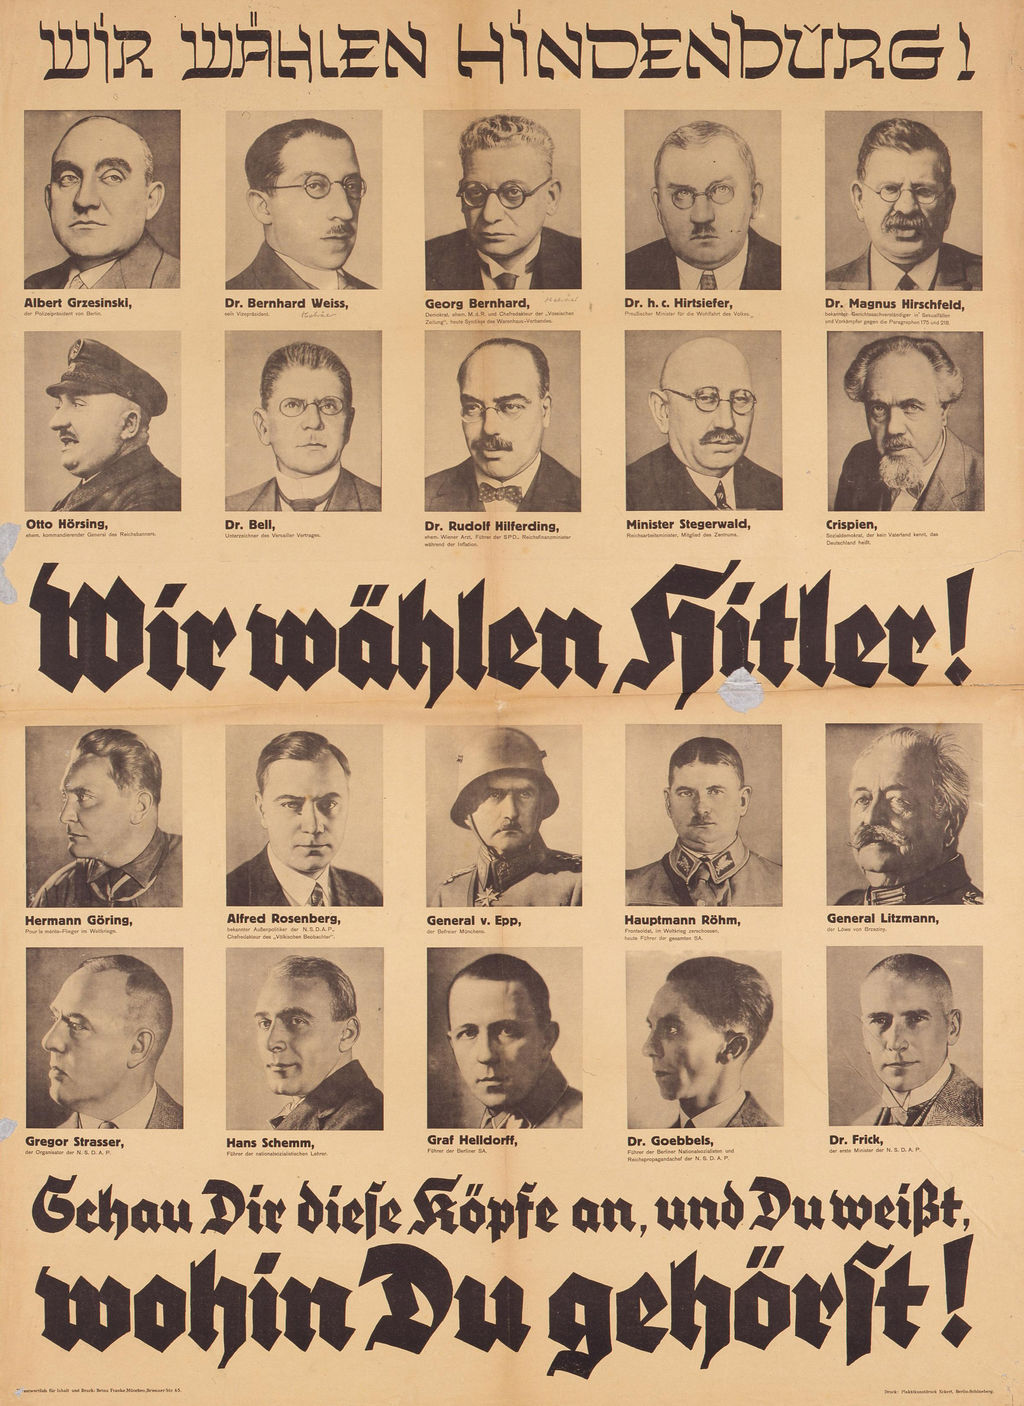
\includegraphics[width=.9\linewidth]{./rassenlehre.jpg}
\end{center}
\end{center}
\newpage
\section{Rassentheorien und Rassenhygiene}
\label{sec:org4a3f88c}
\begin{itemize}
\item grundlegende "`Wissenschaften"'
\item Antisemitismus 19. Jahrhundert
\item Judentum sei keine Religion sondern "`fremdartige und minderwertige Rasse"' (Wilhelm Marr)
\item Rassismus
\end{itemize}

\section{Rassenlehre gegen Juden}
\label{sec:org2d17a90}
\begin{itemize}
\item Hauptfeind der Nazies
\item begann aber schon Früher
\item Martin Luther (1545):  „Von den Juden und ihren Lügen“
\end{itemize}
\end{document}
